\documentclass[../../main.tex]{subfiles}
\begin{document}

{\bf [解答]}

\begin{figure}[htb]
  \centering
  \begin{tikzpicture}[x=1.25cm, y=1.2cm, every node/.style={font=\small}]
    % Congruent illustrative triangles ensure AB=DE and equal r,R.
    \begin{scope}
      \coordinate (A) at (0,2.4);
      \coordinate (B) at (-2,0);
      \coordinate (C) at (2,0);
      \coordinate (O) at (0,0.937);
      \coordinate (Oc) at (0,0.3667);
      \coordinate (Hab) at ($(A)!(O)!(B)$);
      \coordinate (Hbc) at (0,0);
      \coordinate (Hca) at ($(A)!(O)!(C)$);
      \begin{scope}
        \clip (-2.35,-0.32) rectangle (2.35,2.65);
        \draw[gray!60, thick] (Oc) circle[radius=2.033];
      \end{scope}
      \draw[line width=1.3pt, blue!85!black] (A)--(B)--(C)--cycle;
      \draw[dashed, gray!65] (A)--(O) (B)--(O) (C)--(O);
      \draw[thick, teal!75!black] (O) circle[radius=0.937];
      \draw[dashed, red!75!black] (O)--(Hab) (O)--(Hbc) (O)--(Hca);
      % \draw[dashed, orange!80!black] (Oc)--(C);
      \node[circle, fill, inner sep=1.3pt] at (A) {}; \node[above=2pt] at (A) {$A$};
      \node[circle, fill, inner sep=1.3pt] at (B) {}; \node[below left=2pt] at (B) {$B$};
      \node[circle, fill, inner sep=1.3pt] at (C) {}; \node[below right=2pt] at (C) {$C$};
      \node[circle, fill=red!80!black, inner sep=1.1pt] at (Hab) {};
      \node[above left=1pt, font=\footnotesize, red!80!black] at (Hab) {$H_{ab}$};
      \node[circle, fill=red!80!black, inner sep=1.1pt] at (Hbc) {};
      \node[below=2pt, font=\footnotesize, red!80!black] at (Hbc) {$H_{bc}$};
      \node[circle, fill=red!80!black, inner sep=1.1pt] at (Hca) {};
      \node[above right=1pt, font=\footnotesize, red!80!black] at (Hca) {$H_{ca}$};
      \node[circle, fill=teal!80!black, inner sep=1.3pt] at (O) {}; \node[teal!80!black, above right=2pt] at (O) {$O$};
      % \node[circle, fill=orange!80!black, inner sep=1.1pt] at (Oc) {}; \node[orange!80!black, left=3pt, font=\footnotesize] at (Oc) {$O'$};
      \node[red!80!black, font=\footnotesize] at (0.18,0.46) {$r$};
      \node[orange!80!black, font=\footnotesize] at (1.24,0.43) {$R$};
      \node[font=\footnotesize] at (-0.25,1.9) {$\alpha$};
      \node[font=\footnotesize] at (-1.55,0.28) {$\beta$};
      \node[font=\footnotesize] at (1.55,0.28) {$\gamma$};
    \end{scope}
    \begin{scope}[shift={(5.3,0)}]
      \coordinate (D) at (0,2.4);
      \coordinate (E) at (-2,0);
      \coordinate (F) at (2,0);
      \coordinate (Oi) at (0,0.937);
      \draw[line width=1.3pt, blue!85!black] (D)--(E)--(F)--cycle;
      \draw[dashed, gray!65] (D)--(Oi) (E)--(Oi) (F)--(Oi);
      \draw[thick, teal!75!black] (Oi) circle[radius=0.937];
      \node[circle, fill, inner sep=1.3pt] at (D) {}; \node[above=2pt] at (D) {$D$};
      \node[circle, fill, inner sep=1.3pt] at (E) {}; \node[below left=2pt] at (E) {$E$};
      \node[circle, fill, inner sep=1.3pt] at (F) {}; \node[below right=2pt] at (F) {$F$};
      \node[circle, fill=teal!80!black, inner sep=1.3pt] at (Oi) {}; \node[teal!80!black, above right=2pt] at (Oi) {$O'$};
      \node[font=\footnotesize] at (-0.25,1.9) {$\alpha'$};
      \node[font=\footnotesize] at (-1.55,0.28) {$\beta'$};
      \node[font=\footnotesize] at (1.55,0.28) {$\gamma'$};
    \end{scope}
  \end{tikzpicture}
  \caption{二つの三角形の内心と垂線の足 $H_{ab},H_{bc},H_{ca}$ および半角 $\alpha,\beta,\gamma$，$\alpha',\beta',\gamma'$}
  \label{fig:1963_2_triangles}
\end{figure}

$\triangle ABC, \triangle DEF$の内接円の半径 $r$, 外接円の半径 $R$ とおく．
$\triangle ABC$ において内心 $O$ とし，図のように角度を
\begin{align}
  \begin{cases}
    \angle OAB = \alpha, \angle OBC = \beta, \angle OCA = \gamma \\
    \alpha+\beta+\gamma = \dfrac{\pi}{2}
  \end{cases} \label{eq:1}
\end{align}
とおく．
また内心$O$から辺$AB,BC,CA$に下ろした垂線の足を$H_{ab},H_{bc},H_{ca}$とおく．

全く同様に$\triangle DEF$ において内心 $O'$ とし，図のように角度を
\begin{align}
  \begin{cases}
    \angle O'A'B' = \alpha', \angle O'B'C' = \beta', \angle O'C'A' = \gamma' \\
    \alpha'+\beta'+\gamma' = \dfrac{\pi}{2}
  \end{cases} \label{eq:2}
\end{align}
とプライムをつけて表す．$\{\alpha, \beta, \gamma\} = \{\alpha', \beta', \gamma'\}$，すなわち$\{\alpha, \beta\} = \{\alpha', \beta'\}$ ならば $\triangle ABC$ と $\triangle DEF$ は合同である．

まず$\triangle ABC$について考える．
辺$AB$の長さは
\begin{align}
  |AB| = |AH_{ab}| + |BH_{ab}| = \dfrac{r}{\tan \alpha} + \dfrac{r}{\tan \beta}
\end{align}
だから正弦定理から
\begin{align}
  \dfrac{|AB|}{\sin \angle ACB} = 2R
  \quad \therefore
  \dfrac{r}{\sin 2\gamma} \left( \dfrac{1}{\tan \alpha} + \dfrac{1}{\tan \beta} \right) = 2R
\end{align}
となる．整理して
\begin{align}
  & \dfrac{r}{\sin 2\gamma} \left( \dfrac{\cos \alpha}{\sin \alpha} + \dfrac{\cos \beta }{\sin \beta} \right) = \dfrac{2R}{r} \\
  & \dfrac{\cos\alpha\sin\beta + \cos\beta\sin\alpha }{\sin 2\gamma \sin \alpha \sin \beta } = \dfrac{2R}{r} \\
  & \dfrac{\sin(\alpha+\beta)}{2 \sin\gamma\cos\gamma \sin \alpha \sin \beta } = \dfrac{2R}{r} \\
  & \dfrac{\sin(\alpha+\beta)}{\cos\gamma}\dfrac{1}{\sin\gamma \sin \alpha \sin \beta } = \dfrac{4R}{r}
\end{align}
であり，\cref{eq:1}より$\sin(\alpha+\beta) = \sin(\pi/2-\gamma) = \cos \gamma$ だから
\begin{align}
  \sin\gamma \sin \alpha \sin \beta = \dfrac{r}{4R} \label{eq:3}
\end{align}
である．全く同様に$\triangle DEF$ について
\begin{align}
  \sin \alpha' \sin \beta' \sin \gamma' = \dfrac{r}{4R} \label{eq:4}
\end{align}
が成り立つ．\cref{eq:3,eq:4}が成り立つ時に$\{\alpha, \beta\} = \{\alpha', \beta'\}$ が成り立つかを調べる．\cref{eq:1}より$\gamma=\dfrac{\pi}{2}-\alpha-\beta$などを代入して
\begin{align}
  \sin \alpha \sin \beta \sin\left(\dfrac{\pi}{2}-\alpha-\beta\right)
  =\sin \alpha' \sin \beta' \sin\left(\dfrac{\pi}{2}-\alpha'-\beta'\right)
  =\dfrac{r}{4R}
\end{align}
だから，
\begin{align}
  f(x, y)
  &= \sin x \sin y \sin(\pi/2 - x - y) \\
  &= \sin x \sin y \cos(x+y) \quad (0 < x, y, \ x+y < \pi/2) \label{eq:5}
\end{align}
とおくと，
\begin{align}
  f(\alpha,\beta) = f(\alpha',\beta') = \dfrac{r}{4R} \label{eq:6}
\end{align}
である．
そこで$f(x,y)$のとりうる値を考える．もし，異なる2組の $(x,y)$ に対し $f(x,y)$ が同じ値をとるなら，$\triangle ABC$ と $\triangle DEF$ は合同とは限らない．

積和の公式から
\begin{align}
  f(x,y) = \dfrac{1}{2} \sin y \{ \sin(2x+y) - \sin y \}
\end{align}
である．

\begin{figure}[htb]
  \centering
  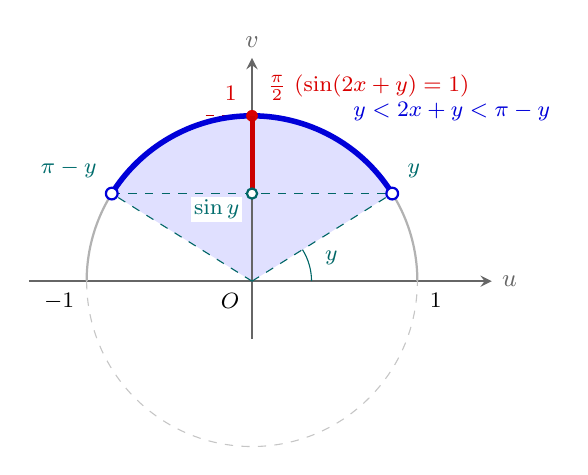
\begin{tikzpicture}[x=2.1cm, y=2.1cm, >=stealth, every node/.style={font=\small}]
    % Illustrative angle y = 32 deg (0 < y < pi/2)
    \pgfmathsetmacro{\angy}{32}
    \pgfmathsetmacro{\cy}{cos(\angy)}
    \pgfmathsetmacro{\sy}{sin(\angy)}
    \coordinate (O) at (0, 0);
    \coordinate (Py) at (\cy, \sy);
    \coordinate (Ppiy) at (-\cy, \sy);
    \coordinate (Ptop) at (0, 1);

    % 扇形の淡い塗り (y < 2x+y < pi-y)
    \fill[blue!12] (O) -- (Py) arc[start angle=\angy, end angle={180-\angy}, radius=1] -- cycle;

    % 座標軸と単位円
    \draw[->, thick, gray!80!black] (-1.35, 0) -- (1.45, 0) node[right] {$u$};
    \draw[->, thick, gray!80!black] (0, -0.35) -- (0, 1.35) node[above] {$v$};
    \draw[thick, gray!60] (1, 0) arc[start angle=0, end angle=180, radius=1];
    \draw[dashed, gray!45] (-1, 0) arc[start angle=180, end angle=360, radius=1];

    % 動径と高さ sin y の破線
    \draw[dashed, teal!80!black] (O) -- (Py);
    \draw[dashed, teal!80!black] (O) -- (Ppiy);
    \draw[dashed, teal!80!black] (Ppiy) -- (Py);
    \draw[dashed, red!75!black] (-0.28, 1) -- (Ptop);

    % 角度 y の弧
    \draw[thin, teal!80!black] (0.36, 0) arc[start angle=0, end angle=\angy, radius=0.36];
    \node[font=\footnotesize, teal!80!black] at (0.48, 0.14) {$y$};

    % 円周上の範囲 y < 2x+y < pi-y (太い青弧 + 両端白抜き)
    \draw[line width=2.0pt, blue!85!black] (Py) arc[start angle=\angy, end angle={180-\angy}, radius=1];
    \node[circle, draw=blue!85!black, thick, fill=white, inner sep=1.5pt] at (Py) {};
    \node[circle, draw=blue!85!black, thick, fill=white, inner sep=1.5pt] at (Ppiy) {};

    % 最大点 2x+y = pi/2
    \node[circle, fill=red!85!black, inner sep=1.5pt] at (Ptop) {};
    \node[above right=2pt, font=\footnotesize, red!85!black] at (Ptop) {$\frac{\pi}{2}\ (\sin(2x+y)=1)$};

    % sin(2x+y) の範囲を y 軸上に強調
    \draw[line width=1.8pt, red!80!black] (0, \sy) -- (0, 1);
    \node[circle, draw=teal!80!black, thick, fill=white, inner sep=1.3pt] at (0, \sy) {};

    % ラベル
    \node[above right=2pt, font=\footnotesize, teal!85!black] at (Py) {$y$};
    \node[above left=2pt, font=\footnotesize, teal!85!black] at (Ppiy) {$\pi-y$};
    \node[above right=2pt, font=\footnotesize, blue!85!black] at (0.52, 0.88) {$y < 2x+y < \pi-y$};
    \node[below left=1pt, font=\footnotesize, teal!85!black, fill=white, inner sep=1pt] at (-0.04, \sy) {$\sin y$};
    \node[above left=2pt, font=\footnotesize, red!85!black] at (Ptop) {$1$};
    \node[below right=1pt, font=\footnotesize] at (1, 0) {$1$};
    \node[below left=1pt, font=\footnotesize] at (-1, 0) {$-1$};
    \node[below left=1pt, font=\footnotesize] at (O) {$O$};
  \end{tikzpicture}
  \caption{$0<y<\dfrac{\pi}{2}$ を固定したときの $y < 2x+y < \pi-y$ の単位円周上の範囲と $\sin y < \sin(2x+y) \le 1$}
  \label{fig:1963_2_unit_circle}
\end{figure}

まず $y$ を固定して考える．$0 < x < \pi/2$ から $y < 2x+y < \pi-y$, $0 < y < \pi/2$ に注意して$2x+y=\pi/2$なる$x$が必ずあるから
\begin{align}
  0 < f(x,y) \le \dfrac{1}{2} \sin y (1 - \sin y) \label{eq:7}
\end{align}
となる．

次に $t = \sin y \ (0 < t < 1)$ とおいて，$y$ をうごかすことにより $S = \max_{x} f(x,y)$ のとりうる領域は図の色付き部分である（境界は，斜線部のみ含む）．

\begin{figure}[htb]
  \centering
  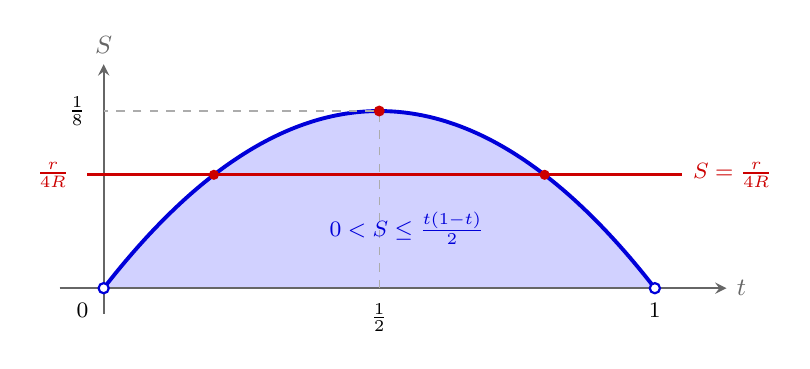
\begin{tikzpicture}[x=7cm, y=18cm, >=stealth,
    every node/.style={font=\small}]
    % S ranges over 0<S<=t(1-t)/2 with 0<t<1.
    \fill[blue!18] (0,0)
    -- plot[domain=0:1, samples=100] (\x,{0.5*\x*(1-\x)})
    -- (1,0) -- cycle;
    \draw[->, thick, gray!80!black] (-0.08,0) -- (1.13,0)
    node[right] {$t$};
    \draw[->, thick, gray!80!black] (0,-0.018) -- (0,0.158)
    node[above] {$S$};
    \draw[line width=1.4pt, blue!85!black, domain=0:1,
    samples=100, smooth] plot (\x,{0.5*\x*(1-\x)});
    \draw[dashed, gray!65] (0.5,0)--(0.5,0.125)--(0,0.125);
    % S = r/(4R) の直線 (0 < r/(4R) < 1/8 の例: S = 0.08)
    \draw[line width=1.1pt, red!80!black] (-0.03,0.08) -- (1.05,0.08)
    node[right, font=\footnotesize] {$S=\frac{r}{4R}$};
    \node[circle, fill=red!80!black, inner sep=1.3pt] at ({0.5-sqrt(0.09)},0.08) {};
    \node[circle, fill=red!80!black, inner sep=1.3pt] at ({0.5+sqrt(0.09)},0.08) {};
    \node[circle, fill=red!80!black, inner sep=1.4pt] at (0.5,0.125) {};
    \node[circle, draw, thick, blue!85!black, fill=white, inner sep=1.3pt] at (0,0) {};
    \node[circle, draw, thick, blue!85!black, fill=white, inner sep=1.3pt] at (1,0) {};
    \node[below left=2pt, font=\footnotesize] at (0,0) {$0$};
    \node[below=2pt, font=\footnotesize] at (0.5,0) {$\frac{1}{2}$};
    \node[below=2pt, font=\footnotesize] at (1,0) {$1$};
    \node[left=3pt, font=\footnotesize] at (0,0.125) {$\frac{1}{8}$};
    \node[left=3pt, font=\footnotesize, red!80!black] at (-0.03,0.08) {$\frac{r}{4R}$};
    \node[blue!85!black, font=\footnotesize] at (0.55,0.042)
    {$0<S\le\frac{t(1-t)}{2}$};
  \end{tikzpicture}
  \caption{$t=\sin y$ に対する $S=f(x,y)$ の値域と直線 $S=\dfrac{r}{4R}$ の共有点}
  \label{fig:1963_2_range}
\end{figure}

特に境界$S=t(1-t)/2$においては$0<y<\pi/2より$t$に対して$yが一つ対応し，それに応じて$2x+y=\pi/2$から$x$が一意に定まる．特に$t=1/2$の時は$y=x=\pi/6$が唯一対応する．

従ってこの領域と$y=\dfrac{r}{4R}$の交点を考えて，
\begin{align}
  \begin{cases}
    0 < \dfrac{r}{4R} < \dfrac{1}{8} \text{ の時，合同とは限らない} \\
    \dfrac{r}{4R} = \dfrac{1}{8} \text{ の時，合同}
  \end{cases}
\end{align}
である．

\newpage

\end{document}
